\documentclass[11pt,a4paper]{article}

% Encodage et langue
\usepackage[utf8]{inputenc}
\usepackage[T1]{fontenc}
\usepackage[english]{babel}

% Maths et mise en page
\usepackage{amsmath, amssymb}
\usepackage{geometry}
\geometry{margin=2.5cm}
\usepackage{indentfirst}

% Images et liens
\usepackage{graphicx}
\usepackage{hyperref}
\usepackage{tikz}
\usetikzlibrary{trees, positioning}



% Infos document
\title{MCTS Project}
\author{
Gabriella FERNANDES MACEDO \\
Ruben IFRAH \\
}
\date{}

\begin{document}

\maketitle


\tableofcontents

\newpage

\section{Motivation: Why Combine MCTS and SINDy?}
\label{sec:motivation}

The fundamental goal of Symbolic Regression (SR) is to automatically discover mathematical equations that govern a dataset. Traditionally, this is achieved either through evolutionary algorithms (like Genetic Programming) or through sparse regression over a predefined dictionary of functions (like SINDy). However, both approaches suffer from fatal scaling barriers when applied to highly complex dynamical systems. The proposed hybrid MCTS-SINDy architecture is specifically designed to bypass these two distinct barriers.

\subsection{The Continuous Optimization Bottleneck of Standard SR}
In traditional grammar-guided Symbolic Regression (such as the original Symbolic Physics Learner), the agent builds a complete algebraic equation tree that includes numerical constants (e.g., $c_0 \sin(x) + c_1 y$). Evaluating the fitness of this tree requires running a continuous, non-convex numerical optimizer (like BFGS or Powell) at the leaf nodes to fit these constants to the data. 

This optimization step is computationally devastating. The loss landscapes of arbitrary non-linear equations are riddled with local minima, causing optimizers to fail or take thousands of iterations to converge. This makes standard SR insurmountably slow when scaling to complex multivariate problems.

\subsection{The Combinatorial Explosion of Pure SINDy}
The SINDy algorithm elegantly solves the constant-fitting problem by framing it as a sparse linear regression task ($\dot{X} = \mathbf{\Theta}(X) \mathbf{\Xi}$). Because it uses Sequentially Thresholded Least Squares (STLSQ) or LASSO, calculating the coefficients $\mathbf{\Xi}$ is practically instantaneous and mathematically convex.

However, pure SINDy relies on a \textit{static, predefined} library of candidate features $\mathbf{\Theta}(X)$ (typically low-degree polynomials and trigonometrics). This works perfectly for simple, well-known systems like the Lorenz attractor. But consider a physical system governed by a deeply nested, highly non-linear term, such as:
\begin{equation}
    \dot{x} = \frac{\sin(x^2 \cdot y)}{1 + \exp(-z)}
\end{equation}

To guarantee that a static dictionary simply \textit{contains} this specific basis function, the researcher would have to forcefully pre-compute every possible mathematical combination of operators ($\sin, \cos, \exp, +, -, *, /$) and variables ($x, y, z$) up to depth 6 or 7. Due to the exponential branching factor of mathematical grammars, a depth-7 library consists of millions or billions of generated terms.

Passing a matrix with $p = 1,000,000$ columns and $n = 1,000$ data points to a regression solver creates a massively ill-posed problem ($p \gg n$). The matrices become perfectly singular, STLSQ fails to converge, and the computer runs out of RAM. In short, pure SINDy cannot discover novel governing equations unless the human operator already intuitively knows what non-linear shapes to manually code into the dictionary.

\subsection{The Hybrid Solution: Dynamic Memory-Efficient Filtering}
The integration of Monte Carlo Tree Search provides the definitive solution to the dictionary explosion problem. MCTS acts as a \textbf{dynamic, memory-efficient filter} across the infinite grammar space.

Instead of instantiating 1 billion columns in RAM, the MCTS heuristic traverses the infinite mathematical tree and selectively passes only small, focused feature matrices (e.g., 5 to 10 dynamically generated columns at a time) to SINDy. By leveraging rigorous selection metrics like the Bayesian Information Criterion (BIC), the MCTS is heavily penalized for exploring garbage branches. This feedback loop allows the agent to autonomously "snipe" the exact non-linear features required to explain the data without ever triggering a dense matrix collapse.

In summary, while using an MCTS to discover simple linear relationships (like $\dot{x} = -0.1x + y$) may feel like overkill compared to static dictionaries, the hybrid architecture is strictly necessary to unlock the autonomous AI discovery of highly nested, counter-intuitive governing equations in fields like fluid dynamics or quantum mechanics that humans have not yet conceptualized.

\section{Reward Function Design and Optimization Strategy}
\label{sec:reward_design}

The design of the reward function is the most critical component of the Monte Carlo Tree Search (MCTS) architecture, as it provides the sole feedback signal guiding the agent's exploration of the combinatorial grammar space. Our objective is to discover governing physical equations that are both highly accurate and parsimonious. In this section, we detail the evolution of the reward formulation, transitioning from a standard additive penalty model to a robust, information-theoretic framework integrated with sparse regression.

\subsection{The Baseline Formulation and its Limitations}
Standard grammar-guided symbolic regression frameworks, such as the Symbolic Physics Learner (SPL), evaluate generated expression trees using numerical optimizers (e.g., the Powell method or BFGS) at the leaf nodes to estimate continuous constants. The fitness of a complete tree is typically evaluated using a baseline reward function that balances the Mean Squared Error (MSE) with a structural parsimony penalty:

\begin{equation}
    \mathcal{R}_{\text{baseline}} = \frac{\eta^n}{1 + \text{MSE}}
\end{equation}

where $\eta \in (0, 1)$ is a discount factor and $n$ represents the total number of production rules utilized to construct the tree. While intuitive, this approach suffers from severe computational bottlenecks due to the non-convex nature of the continuous parameter optimization, and it struggles to scale to complex dynamical systems.

\subsection{Transition to a Hybrid MCTS-SINDy Architecture}
To overcome the computational limitations of non-convex optimization, we propose a hybrid architecture where MCTS acts as a \textit{feature generator} rather than a strict equation builder. The MCTS explores the syntax tree to organically construct a library of candidate nonlinear basis functions, $\mathbf{\Phi}(X) = [\phi_1(X), \phi_2(X), \dots, \phi_m(X)]$. 

This generated library is then passed to a Sequentially Thresholded Least Squares (STLSQ) solver, akin to the SINDy algorithm. The solver instantly computes a sparse vector of coefficients $\mathbf{\Xi}$, forcing the coefficients of redundant or non-governing features to exactly zero. Consequently, the reward function must be redesigned to evaluate not just a single tree, but the performance of the surviving terms within the feature matrix.

\subsection{The Intermediate Additive Penalty Reward}
In the hybrid paradigm, the reward must penalize complexity, but crucially, it must differentiate between terms that are actively utilized by the STLSQ solver and those that are discarded. An initial proposed formulation for the hybrid reward is an additive model:

\begin{equation}
    \mathcal{R}_{\text{additive}} = \frac{1}{1 + \text{MSE} + \lambda \|\mathbf{\Xi}\|_0 + \alpha \mathcal{C}_{\text{active}} + \beta \mathcal{C}_{\text{unused}}}
\end{equation}

This formulation introduces four competing forces:
\begin{itemize}
    \item \textbf{Data Fidelity ($\text{MSE}$):} The reconstruction error achieved by the STLSQ solver.
    \item \textbf{Sparsity ($\|\mathbf{\Xi}\|_0$):} The $L_0$ norm, directly penalizing the count of non-zero coefficients.
    \item \textbf{Active Complexity ($\mathcal{C}_{\text{active}}$):} A heavy structural penalty ($\alpha$) applied to the grammar depth of the specific features where $\Xi_i \neq 0$.
    \item \textbf{Unused Complexity ($\mathcal{C}_{\text{unused}}$):} A minor structural penalty ($\beta$) applied to generated features that the solver assigned a coefficient of zero.
\end{itemize}

A fundamental constraint in this design is that $\beta \ll \alpha$. If $\beta$ is too large, the MCTS agent becomes risk-averse, proposing only trivial terms to avoid penalties. Conversely, if $\beta = 0$, the agent exploits the solver by proposing infinitely wide feature matrices, leading to ill-conditioned inverse problems. A small $\beta$ acts as a necessary regularizer, encouraging broad exploration while penalizing gratuitous computational bloat.

\subsection{Final Formulation: Information Theory}
While the additive reward conceptually bridges tree search and sparse regression, it is mathematically flawed due to scaling discrepancies. The MSE can vary by orders of magnitude across different equations, making the linear sparsity penalty ($\lambda \|\mathbf{\Xi}\|_0$) highly unstable and hyperparameter-dependent.

To establish a mathematically rigorous selection criterion, we abandon the linear combination in favor of the Bayesian Information Criterion (BIC). BIC leverages logarithmic scaling to inherently balance the maximum likelihood of the model against its dimensionality:

\begin{equation}
    \text{BIC} = n \ln(\text{MSE}) + \|\mathbf{\Xi}\|_0 \ln(n)
\end{equation}

where $n$ is the number of data points. To integrate BIC into the MCTS framework—which requires a bounded reward signal $\mathcal{R} \in (0, 1]$ to maintain calibrated Upper Confidence Bounds (UCT)—we apply an exponential decay to the BIC score, while retaining the structural syntax penalties in the denominator. This yields our final, state-of-the-art reward formulation:

\begin{equation}
    \mathcal{R}_{\text{final}} = \exp(-\gamma \cdot \text{BIC}) \times \frac{1}{1 + \alpha \mathcal{C}_{\text{active}} + \beta \mathcal{C}_{\text{unused}}}
\end{equation}

where $\gamma$ scales the sensitivity of the exponential. This formulation represents a significant advancement over standard symbolic regression rewards. The numerator statistically guarantees that the MCTS is rewarded for discovering the true governing dynamics without overfitting, while the denominator ensures the mathematical elegance of the underlying syntax tree.

\subsection{Structural Complexity and the Hyperparameter Dichotomy}
To fully realize the benefits of the hybrid architecture, the denominator of the reward function meticulously decouples the structural complexity of the generated grammar tree into two distinct components: active and unused features. 

Let the MCTS agent generate a candidate library comprised of $m$ features, $\mathbf{\Phi} = \{\phi_1, \phi_2, \dots, \phi_m\}$. For each feature $\phi_i$, we define its individual structural complexity, $c(\phi_i)$, as the number of discrete production rules required to derive it from the underlying context-free grammar. Upon evaluation by the STLSQ solver, the features are partitioned based on their corresponding sparse coefficients in $\mathbf{\Xi}$:

\begin{itemize}
    \item \textbf{Active Complexity ($\mathcal{C}_{\text{active}}$):} The sum of grammatical complexities for all features retained by the solver: 
    \begin{equation}
        \mathcal{C}_{\text{active}} = \sum_{i : \Xi_i \neq 0} c(\phi_i)
    \end{equation}
    \item \textbf{Unused Complexity ($\mathcal{C}_{\text{unused}}$):} The sum of grammatical complexities for all features successfully pruned by the solver: 
    \begin{equation}
        \mathcal{C}_{\text{unused}} = \sum_{j : \Xi_j = 0} c(\phi_j)
    \end{equation}
\end{itemize}

A fundamental mathematical constraint for this reward architecture is the strict inequality $\beta \ll \alpha$. This dichotomy resolves the inherent tension between combinatorial exploration and physical parsimony. 

If $\beta$ were assigned a weight comparable to $\alpha$, the MCTS agent would become highly risk-averse. To avoid severe penalties for generating terms that SINDy might ultimately reject, the optimal policy would collapse into proposing only trivial, low-complexity features (e.g., standard linear variables), effectively neutralizing the MCTS's ability to discover complex, nested dynamics. Conversely, setting $\beta = 0$ removes all friction from generation, allowing the agent to propose infinitely wide feature matrices. This causes the STLSQ optimization to become statistically ill-posed ($p \gg n$) and computationally unstable.

By enforcing $\beta \ll \alpha$, the reward acts as a mild "generation tax." It encourages the MCTS to function as a highly exploratory brainstorming engine—freely proposing highly non-linear, complex basis functions that bypass human bias—while relying on the heavy $\alpha$ penalty to enforce Occam's razor strictly on the final, physically governing terms.


The exponential transformation, $\exp(-\gamma \cdot \text{BIC})$, is a critical adaptation for integrating statistical model selection into a Reinforcement Learning paradigm. Raw Information Criteria can span wide, unbounded numerical ranges depending on the variance of the underlying dataset. Directly backpropagating such unbounded error signals inevitably destabilizes the Upper Confidence Bound (UCT) equation used during the MCTS selection phase.

The hyperparameter $\gamma$ acts as a temperature scaling factor, compressing the unbounded BIC score into a strictly bounded probability-like domain $(0, 1]$. Consequently, the MCTS agent optimizes over a smooth, normalized manifold. This mathematical synthesis guarantees that the search tree reliably converges toward the Pareto front of models—simultaneously maximizing data likelihood while minimizing both continuous parameter counts and discrete syntactical complexity.

\section{Grammar and Tree Construction}
\label{sec:grammar_tree}

The foundation of the MCTS Equation Discovery engine relies on a formal Context-Free Grammar (CFG). Unlike traditional Symbolic Regression that builds a single global algebraic equation (often struggling with optimization of constants), our modified grammar is intrinsically designed to output a \textit{Library of Features}. This decouples the mathematical shape discovery (handled by MCTS) from the linear coefficient optimization (handled by PySINDy).

\subsection{Production Rules}
The grammar consists of a set of Non-Terminals ($\mathcal{N}$), Terminals ($\mathcal{T}$), and Production Rules ($\mathcal{P}$). The generation always begins with the root symbol $f$.
\begin{itemize}
    \item $\mathcal{N} = \{f, \text{Library}, \text{Feature}, M\}$
    \item $\mathcal{T} = \{x, y, z, *, \sin, \cos, \exp\}$
\end{itemize}

The core production rules are defined as follows:
\begin{align*}
    f &\rightarrow \text{Library} \\
    \text{Library} &\rightarrow \text{Feature} \\
    \text{Library} &\rightarrow \text{Feature}, \text{Library} \\
    \text{Feature} &\rightarrow M \\
    M &\rightarrow M * M \mid \sin(M) \mid \cos(M) \mid \exp(M) \mid x \mid y \mid z
\end{align*}

This recursive definition is crucial: the \texttt{Library} rule allows the MCTS to dynamically dictate the width of the feature matrix prior to calculating the internal physics of each term. This replaces the rigid "+ / -" operators found in standard equation trees.

\subsection{LIFO Stack Mechanics}
The MCTS builds the tree sequentially by maintaining a Last-In, First-Out (LIFO) stack of non-terminals. The process begins with the root symbol \texttt{f} heavily anchoring the stack. At each step, the agent pops the top non-terminal, selects an applicable production rule, and pushes any newly generated non-terminals onto the stack from right to left (ensuring the leftmost symbol is always expanded next).

Understanding the roles of the specific nodes:
\begin{itemize}
    \item \texttt{f}: The mandatory starting root. It immediately forces the creation of a \texttt{Library}.
    \item \texttt{Library}: Dictates the width of the final equation matrix. Calling $\text{Library} \rightarrow \text{Feature}, \text{Library}$ adds a new column to the PySINDy matrix, whereas $\text{Library} \rightarrow \text{Feature}$ terminates the matrix expansion.
    \item \texttt{Feature}: An isolation wrapper. It guarantees that the mathematical expression generated underneath it remains a distinct, separable term to be plugged into SINDy, rather than merging algebraically with other terms.
    \item \texttt{M}: The core math generator. It recursively stacks operators ($\sin, \cos, *, \dots$) and terminates with variables ($x, y, z$).
\end{itemize}

\subsection{AST Construction Example}
Consider the exact sequence of rules chosen to generate Figure \ref{fig:ast_example}: a library containing two features $[\phi_1 = x, \phi_2 = \sin(y)]$. The step-by-step mechanics unfold as follows:

\begin{enumerate}
    \item \textbf{Initialize:} Stack $= [f]$
    \item \textbf{Rule $f \rightarrow \text{Library}$:} Pop $f$, push $\text{Library}$.\\
          \textit{Stack} $= [\text{Library}]$
    \item \textbf{Rule $\text{Library} \rightarrow \text{Feature}, \text{Library}$:} Pop $\text{Library}$, push $\text{Library}$ then $\text{Feature}$. The agent decides the feature matrix will have multiple columns.\\
          \textit{Stack} $= [\text{Feature}, \text{Library}]$
    \item \textbf{Rule $\text{Feature} \rightarrow M$:} Pop $\text{Feature}$, push $M$. We begin building the first basis function.\\
          \textit{Stack} $= [M, \text{Library}]$
    \item \textbf{Rule $M \rightarrow x$:} Pop $M$. As $x$ is a terminal, nothing is pushed.\\
          \textit{Stack} $= [\text{Library}]$
    \item \textbf{Rule $\text{Library} \rightarrow \text{Feature}$:} Pop $\text{Library}$, push $\text{Feature}$. The agent decides this is the final term in the matrix.\\
          \textit{Stack} $= [\text{Feature}]$
    \item \textbf{Rule $\text{Feature} \rightarrow M$:} Pop $\text{Feature}$, push $M$.\\
          \textit{Stack} $= [M]$
    \item \textbf{Rule $M \rightarrow \sin(M)$:} Pop $M$, push $M$. A unary operator is applied.\\
          \textit{Stack} $= [M]$
    \item \textbf{Rule $M \rightarrow y$:} Pop $M$. A terminal is applied.\\
          \textit{Stack} $= []$ (Empty)
\end{enumerate}

When the stack is empty, the sequence is perfectly complete. The parser then extracts all branches originating from a \texttt{Feature} node, resulting in the final abstract syntax tree shown below.

\begin{figure}[htpb]
    \centering
    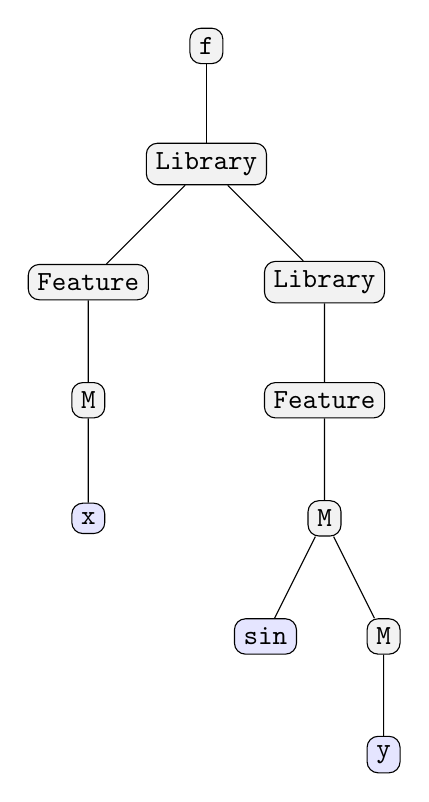
\begin{tikzpicture}[
      level 1/.style={sibling distance=4cm},
      level 2/.style={sibling distance=3cm},
      level 3/.style={sibling distance=1.5cm},
      every node/.style = {shape=rectangle, rounded corners,
        draw, align=center, fill=black!5, font=\ttfamily}
    ]
      \node {f}
        child { node {Library}
          child { node {Feature}
            child { node {M}
              child { node[fill=blue!10] {x} }
            }
          }
          child { node {Library}
            child { node {Feature}
              child { node {M}
                child { node[fill=blue!10] {sin} }
                child { node {M}
                  child { node[fill=blue!10] {y} }
                }
              }
            }
          }
        };
    \end{tikzpicture}
    \caption{Abstract Syntax Tree generated by the modified grammar. The parser recursively traverses the \texttt{Library} nodes to extract the isolated \texttt{Feature} subtrees (shaded path endpoints), ultimately compiling the basis library $\mathbf{\Phi}(X) = [x, \sin(y)]$.}
    \label{fig:ast_example}
\end{figure}

The structural complexity penalties ($\mathcal{C}_{\text{active}}$ and $\mathcal{C}_{\text{unused}}$) introduced in Equation 4 are calculated precisely by counting the number of nodes forming each isolated \texttt{Feature} subtree in this AST.

\section{MCTS Exploration Strategies for Equation Discovery}

\textbf{The Core Problem:} Standard MCTS algorithms were built for spatial board games (Go, Chess). We are building Abstract Syntax Trees (ASTs). Math grammars have massive branching factors ($+$, $*$, $\sin$, $\cos$, $x$, $y$). If the tree goes deep, the combinatorial space explodes.

\subsection*{1. UCT + Uniform Random Rollouts (Current Baseline)}
\begin{itemize}
    \item \textbf{Mechanism:} When reaching an unexpanded node, the agent finishes the equation by picking grammar rules completely at random ($1/N$ probability) until the LIFO stack is empty.
    \item \textbf{Why it fails here:} The probability of a random walk successfully building a specific, physically meaningful 8-deep equation (like a coupled oscillator) is statistically zero. 
    \item \textbf{Result:} The agent wastes 99\% of its SINDy evaluation budget scoring mathematical garbage like $\sin(\exp(\cos(x)))$ instead of exploring broad, simple basis functions.
\end{itemize}

\subsection*{2. AMAF / RAVE (The "Context-Independence" Trap)}
\begin{itemize}
    \item \textbf{Mechanism:} All-Moves-As-First (AMAF). If a move is good, it gets a high score \textit{everywhere} in the tree, regardless of when it was played.
    \item \textbf{Why it fails here:} Math is strictly \textbf{context-dependent}.
    \begin{itemize}
        \item Playing $M \rightarrow \sin(M)$ at the root might yield a huge reward because the data is periodic.
        \item AMAF will globally memorize that "$\sin$ is good" and start blindly injecting it deep inside other branches, like $\exp(\sin(x))$.
    \end{itemize}
    \item \textbf{Result:} AMAF violates the strict topological hierarchy of an Abstract Syntax Tree. It will actively destroy the mathematical structure. Do not use it.
\end{itemize}

\subsection*{3. SHUSS / SHOT (The Best Immediate Upgrade)}
\begin{itemize}
    \item \textbf{Mechanism:} Sequential Halving Applied to Trees. Replaces the blind random rollout with a multi-armed bandit tournament at the decision node.
    \item \textbf{How it works (The Tournament):}
    \begin{enumerate}
        \item At a node with $K$ possible grammar rules, divide the rollout budget equally among all $K$ rules.
        \item Run them, evaluate with SINDy, and \textbf{instantly delete the bottom 50\%} (e.g., throwing out $M \rightarrow M / M$ because it caused a singularity).
        \item Take the remaining budget, redistribute it equally among the surviving 50\%, and repeat until only 1 optimal rule remains.
    \end{enumerate}
    \item \textbf{Why it perfectly fits:} It aggressively prunes bad mathematical operators at the very beginning of the rollout. It forces the compute budget to focus only on structurally sound sub-equations, neutralizing the exponential branching factor.
\end{itemize}

\subsection*{4. PUCT (The Deep Learning / AlphaZero SOTA)}
\begin{itemize}
    \item \textbf{Mechanism:} Predictor + UCT. Replaces uniform rollouts entirely with a trained Neural Network (typically a Transformer).
    \item \textbf{How it works:}
    \begin{itemize}
        \item The network reads the current partial AST.
        \item Outputs a \textbf{Policy} (a rigged probability distribution favoring logical math rules, e.g., heavily biasing $M \rightarrow x$ right after a Feature node to keep the tree shallow).
        \item Outputs a \textbf{Value} (predicting what the SINDy score will be without actually running SINDy).
    \end{itemize}
    \item \textbf{Why it fits:} The network acts as automated "physics intuition." It completely bypasses the combinatorial explosion by looking at a partial equation and knowing instinctively which operators make physical sense next.
\end{itemize}

\vspace{0.5cm}
\noindent \textbf{Actionable Takeaway:} Drop AMAF/RAVE completely. Implement \textbf{SHUSS/SHOT} at the root and deep nodes to efficiently guide the tree generation before the SINDy layer evaluates the library.

\newpage

\section{Limitations of the Current MCTS-SINDy Integration}

While the proposed hybrid approach aims to combine the flexibility of tree-based symbolic exploration with the efficiency of sparse regression, our initial implementation reveals several fundamental limitations. These issues are not merely due to hyperparameter choices but arise from a deeper mismatch between the assumptions of Monte Carlo Tree Search (MCTS) and the structure of the hybrid problem.

\subsection{Mismatch Between MCTS Assumptions and Feature-Based Representation}

In the original Symbolic Physics Learner (SPL), each complete trajectory in the search tree corresponds to a single mathematical expression. As a result, the reward function evaluates a well-defined object, and each decision in the tree directly contributes to constructing that expression.

In contrast, our hybrid approach modifies this paradigm: the MCTS no longer generates a single equation, but instead produces a \textit{library of features} that is subsequently evaluated by a SINDy regression step. The reward is therefore not a function of an individual expression, but of a \textit{set of interacting features}:
\[
\mathcal{R} = f(\phi_1, \phi_2, \dots, \phi_m).
\]

This introduces a critical issue: the contribution of a single feature cannot be evaluated independently. A feature that is useless on its own may become essential when combined with others. For example, in the case of a linear dynamical system such as:
\[
\dot{x} = -0.1x + y,
\]
neither $x$ nor $y$ alone can explain the dynamics accurately, but their combination does. As a result, the MCTS receives low rewards for partial constructions and cannot identify which components are promising.

This phenomenon breaks one of the key assumptions of MCTS: that intermediate decisions can be evaluated through their impact on the final reward. In our setting, the reward is highly non-local and depends on complex interactions between features, making credit assignment extremely difficult.

\subsection{Credit Assignment and Delayed Reward Problem}

The difficulty described above is closely related to the classical credit assignment problem in reinforcement learning. In standard MCTS applications, the reward is observed only at the end of a rollout, but it can still be meaningfully attributed to earlier decisions because the structure being built is coherent and incremental.

In our hybrid setting, however, the reward is produced after a SINDy regression step that may discard most of the generated features. As a consequence:
\begin{itemize}
    \item Features that are not selected by SINDy still influence the reward indirectly.
    \item The MCTS does not observe which features were actually useful.
    \item The same feature may lead to very different rewards depending on the rest of the library.
\end{itemize}

This results in a highly noisy and non-stationary reward signal, which significantly degrades the learning dynamics of the MCTS.

\subsection{Instability Induced by Maximum Reward Backpropagation}

Following SPL, our implementation uses the maximum reward observed during simulations to update node values:
\[
Q(s) \leftarrow \max(Q(s), r).
\]

While this strategy is effective when rewards are stable and directly tied to a single expression, it becomes problematic in our context. Due to the variability introduced by feature interactions and regression, a single high-reward rollout may be the result of a lucky combination rather than a robust pattern. Propagating this maximum value biases the search toward unstable regions of the space and reduces exploration.

In contrast, averaging rewards would provide a more reliable estimate of the expected quality of a node, especially in the presence of stochastic evaluations.

\subsection{Inadequate Complexity Measure}

Another limitation lies in the definition of the structural complexity penalty. In the current implementation, complexity is approximated by the length of the production rule sequence:
\[
\mathcal{C}_{\text{active}} = |\text{sequence}|.
\]

However, this measure does not accurately reflect the true complexity of the generated features. Two sequences of similar length may produce expressions of vastly different interpretability and usefulness. Moreover, this global measure does not distinguish between features that are retained by SINDy and those that are discarded.

As a result, the complexity penalty does not effectively enforce parsimony in the final model.

\subsection{Comparison with the SPL Framework}

These limitations highlight a fundamental difference between our approach and SPL. In SPL:
\begin{itemize}
    \item Each tree corresponds to a single equation.
    \item The reward directly evaluates this equation.
    \item Continuous optimization is used to fit constants within a fixed structure.
\end{itemize}

In our hybrid model:
\begin{itemize}
    \item Each tree generates a set of candidate features.
    \item The final model is obtained through a separate regression step.
    \item The reward evaluates a combination of features rather than a single structured expression.
\end{itemize}

While this design removes the costly continuous optimization step present in SPL, it fundamentally alters the learning problem faced by the MCTS. The search is no longer over self-contained expressions but over sets of interacting components, making the optimization landscape significantly more complex.

\subsection{Summary}

In summary, the current hybrid formulation introduces several challenges:
\begin{itemize}
    \item A non-factorizable reward function depending on feature interactions.
    \item Severe credit assignment issues due to the indirect role of SINDy.
    \item Instability caused by maximum reward backpropagation.
    \item An inadequate measure of structural complexity.
\end{itemize}

These observations suggest that directly combining MCTS and SINDy requires a careful redesign of the reward function and the search strategy. In particular, providing more localized feedback to the MCTS agent and better aligning the representation with the evaluation mechanism appear to be crucial directions for improvement.

\end{document}